% !TEX root = ../master-thesis.tex

% Тут хочется добавить общую последовательность эксперимента. То есть если говорю про imaging with flashing, добавим что происходит с магнитным полем и прочим важным (спросить Намана). Аналогично для state preparation, imaging.

% m: 40-42, 67-70
% h: 84-86, 


\begin{figure}
    \centering
    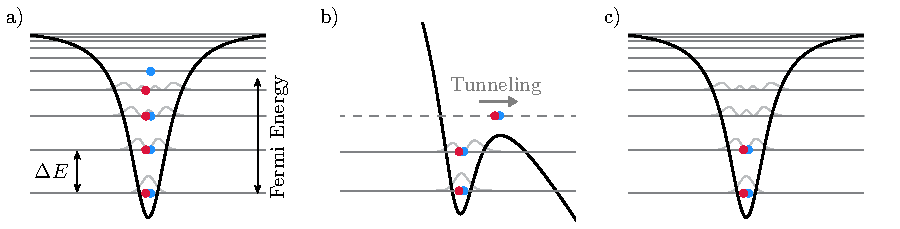
\includegraphics{fig-ai/preparation.pdf}
    \caption{
        \textbf{Deterministic preparation via spilling.}
        (a) Fermionic atoms are initially loaded into a tightly confined optical tweezer, forming a Fermi sea occupying the approximately 1D harmonic oscillator levels up to the Fermi energy. 
        (b) A magnetic field gradient tilts the potential, and the trap depth is lowered such that atoms above a defined spill level tunnel out. 
        (c) This procedure leaves a well-defined number of atoms in the lowest energy states, with a preparation fidelity of approximately 95\%. 
        Blue and red dots denote atoms in different spin states; gray curves indicate the bound-state wavefunctions.
    }
    \label{fig:preparation}
\end{figure}



\textbf{Tweezer loading.} We begin by preparing a spin-balanced mixture in the two lowest hyperfine states, $|1\rangle$ and $|2\rangle$, using a compressed magneto-optical trap (MOT). The atoms are initially loaded into a crossed ODT, where we perform evaporative cooling. This follows closely the sequence described in~\cite{culemann_construction_2024}.

After cooling, the atoms are transferred into a tightly focused optical tweezer potential. The loading process relies on the so-called \emph{dimple trick}~\cite{zurn_few-fermion_2012}, where a tightly confined but deep tweezer potential is superimposed onto the wider ODT reservoir. Because the tweezer affects only a small region of the total cloud, the global temperature $T$ remains approximately unchanged, while the local chemical potential is enhanced. In this regime, the average occupation number $\bar{n}(E_i)$ of a single-particle state $i$ with energy $E_i$ follows the Fermi-Dirac distribution:
\begin{equation}
    \bar{n}(E_i) = \frac{1}{e^{(E_i - \mu)/k_B T} + 1}.
\end{equation}
If the energy gap between the ground state $E_0$ and the Fermi energy $E_F$ is increased such that $(E_0 - E_F) / k_B \gg T$, then $\bar{n}(E_0) \rightarrow 1$. This ensures near-unity occupation of the lowest level, which provides an ideal starting point for deterministic preparation. In our experiment, this condition is achieved by ramping on the tweezer adiabatically while continuing evaporation inside the tweezer. The full loading and cooling sequence is depicted in Fig.~\ref{fig:preparationseq}.

\textbf{Deterministic few-body preparation via spilling.} To isolate a well-defined number of atoms in the lowest motional states of the tweezer, we use the \emph{spilling technique}, as described in~\cite{zurn_few-fermion_2012, holten_pauli_2022}. This method relies on tilting the potential with a magnetic field gradient and reducing the trap depth to allow atoms above a threshold energy to tunnel out. 
The resulting states are shown in Fig.~\ref{fig:preparation}. \red{See Appendix for details.}
% The energy levels and wavefunctions of the effective 1D potential under combined optical and magnetic fields were obtained numerically using a finite-difference method and the Thomas algorithm.

The spilling sequence is performed at a magnetic field of 527\,G, where the two spin states are nearly non-interacting. A magnetic field gradient of 20\,G/cm creates a linear tilt, and the tweezer power is lowered to a value that sets the spill threshold. After a short tunneling time, the trap depth is ramped back up to recapture the remaining atoms. By empirically optimizing these parameters, we achieve deterministic preparation of two atoms per tweezer with a fidelity of approximately 95\,\%. This sequence results in high-fidelity preparation within a total experimental cycle time of less than 2\,s.

% Стоит сказать, что система достаточно симметрична по отношению к уменьшению tweezer depth во время spilling или увеличению градиента. 


\begin{figure}
    \centering
    \addletter{140}{a}
    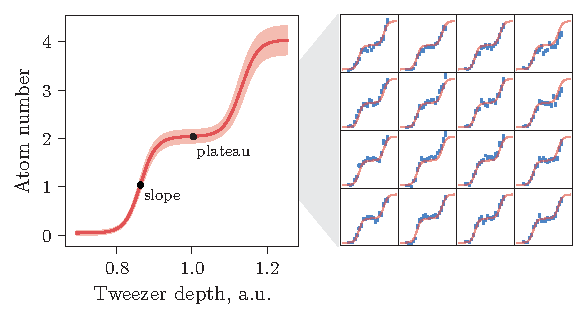
\includegraphics{fig-ai/step-plot-joined.pdf}
    \phantom{42}
    \addletter{140}{b}
    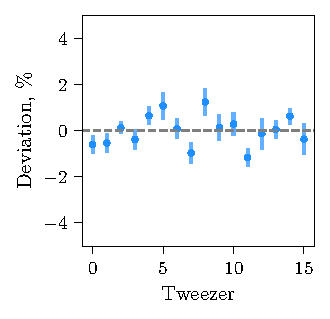
\includegraphics{fig-py/step-plot-balance.pdf} % 0.6 +- 0.2
    % 
    % 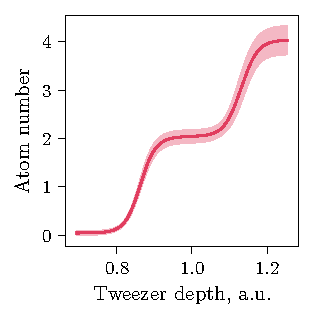
\includegraphics{fig-py/step-plot.pdf}
    % 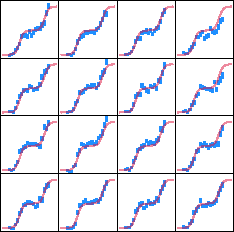
\includegraphics{fig-py/step-plot-inset.pdf}
    \caption{
        \textbf{Step plot.}
        (a) 
        Atom number as a function of tweezer depth during the spilling sequence. 
        % Plateaus correspond to quantized energy levels of the 1D harmonic oscillator. 
        Step plots for each tweezer in the $4 \times 4$ array are shown on the right. The average fit is shown as a solid red line, with standard deviation across sites indicated by the shaded area. 
        (b) Relative deviation of the fitted sigmoid centers for each tweezer after SVF balancing. The standard deviation is $0.7(2)\%$, which is well within the plateau width ($\pm 5\,\%$), ensuring sufficient uniformity for array-wide spilling. \red{$\chi^2$?}
        % All measurements were performed in this work using atom-based measurements and SVF-balanced tweezer depths.
    }
    \label{fig:stepplot}
\end{figure}